
\documentclass[a4paper,10pt,bibtotoc]{scrartcl}
\usepackage{a4wide,usg,supertabular}
\usepackage{draftcopy}

%% Do NOT remove: required to extract SVN information
\svnInfo $Id$

%% Adjust page footer
\fancyfoot[LE,LO]{LOFAR-USG-ICD-007: Visibility Data}
\fancyfoot[RE,RO]{\textsc{lofar} Project}

\begin{document}

%%_______________________________________________________________________________
%% Titlepage

\title{LOFAR Data Format ICD \\ Visibility Data \\
{\normalsize Document ID: LOFAR-USG-ICD-007} \\ 
{\normalsize Version 2.00.03} \\
{\normalsize SVN Repository Revision: \svnInfoMaxRevision}}
\author{K.~Anderson}
\date{\small{SVN Date: \svnInfoMaxToday}}
\maketitle

\tableofcontents

\clearpage

%%_______________________________________________________________________________
%% Change record of the document

\section*{Change record}
\addcontentsline{toc}{section}{Change record}

\begin{center}
  %% Table head
  \tablefirsthead{
    \hline
    \sc Version & \sc Date & \sc Sections & \sc Description of changes \\
    \hline
  }
  \tablehead{
    \multicolumn{4}{r}{\small\sl continued from previous page} \\
    \hline
    \sc Version & \sc Date & \sc Sections & \sc Description of changes \\
    \hline
  }
  %% Table tail
  \tabletail{
    \hline
    \multicolumn{4}{r}{\small\sl continued on next page} \\
  }
  \tablelasttail{\hline}
  %% Table contents
  \begin{supertabular}{lllp{10cm}}
    0.0  & 2010-04-09 & All & Initial revision \\
    0.01 & 2010-04-19 & 4   & Refactor Sec. 4 == 4.1.1 4.1.2 \\
    0.1  & 2010-06-03 & All & Initial commit \\
    0.2  & 2010-06-04 & Appendix & Removed section "Coordinate group examples"
    from the appendix; detailed description and examples now can be found in
    \texttt{LOFAR-USG-ICD-002} ("Representation of World Coordinates") \\
    0.3  & 2010-06-06 & \ref{sec:coordinates group} & Updated description of
    coordinates in order to keep up with changes in \texttt{LOFAR-USG-ICD-002}. \\
    2.00.00  & 2010-07-08 & Cover & Changed `revision` to `version`;  updated 
    this version number to 2.00.00 for LOFAR ICDs 1 through 7 to put them on the same
    version numbering scheme.\\
    2.00.01  & 2011-03-10 & all & Maintain list of references through
    Bib\LaTeX\ database. \\
    2.00.01  & 2011-03-10 & All  & Changed the svnInfoRevision to 
    svnInfoMaxRevision and svnInfoDate to svnInfoMaxToday, in order to take the sub-tex 
    file changes into account for the latex compile.  Added metadata\_intro.tex to explain
    optional vs mandatory keywords. Added several tex import files: version\_numbering, types,
    and notation, just before the Acknowledgements section.  \\
    2.00.03 & 2012-03-06 & cover   & Added draftcopy package for background 'draft' text.\\

  \end{supertabular}
\end{center}

\input version_numbering

\input types

\input notation

\subsection*{Acknowledgements}

\clearpage

%% _______________________________________________________________________________
%% Introduction

\section{Introduction}
\label{sec:introduction}

\subsection{Purpose and Scope}
\label{sec:purpose and scope}

This document sets forth a formal data interface specification for
LOFAR data products.  The specification applies to data structures
produced by various LOFAR processing pipelines that will be called
LOFAR UV Visibility.  This is a specification for LOFAR UV Visibility
data products only and in no way implies, and should not be inferred
as, a specification for any data structures the project may use during
\textit{in situ} processing by way of producing a final standard LOFAR
UV Visibility file.

This document is intended to be the formal interface control agreement
between the LOFAR project, observers/users of LOFAR data products, and
the eventual LOFAR science archive facility.

\subsection{Context and Motivation}
\label{sec:context and motivation}

A LOFAR UV Visibility file will be the data hosting structure for
LOFAR UV Visibility data. It is therefore incumbent on the LOFAR
project to define and describe both the structure of the LOFAR UV
Visibility file format, and the various data types within the context
of that format.

For the LOFAR project, a UV Visibility file product will be defined
within the context of  the Hierarchical Data Format 5, or HDF5. HDF5
allows for  storage, not only of the data, but for the associated and
related meta-data describing the UV Visibility cube contents,
conditions of observations, etc.. As an "all-in-one" wrapper,  HDF5
simplifies the management of what are expected to be very large
datasets that formats such as FITS cannot pragmatically accommodate.

There has been much discussion of a putative need for LOFAR UV
Visibility file headers to adhere to FITS-like header keywords.
Though it is envisioned that the LOFAR project will provide observers
and other users with FITS format files upon request, it is not
entirely necessary that HDF5 header keywords match FITS keyword
conventions in a LOFAR UV Visibility file itself.  A format conversion
layer can certainly be developed to provide rigorous transformation of
LOFAR headers into more restricted FITS header keyword sets.  However,
development of such a layer would be simplified in the event that
LOFAR UV Visibility files make use of \textit{de facto} FITS standard
keywords as much as possible.

For the purposes of further discussion regarding UV Visibility file
adherence to FITS keyword standards, the \textit{ESO Data Interface
  Control Document} (\textit{see \S\ References}), has been adopted as
the FITS keyword model.

\input applicable_documents

%% ______________________________________________________________________________
%%                                                              Section: Overview

\section{Overview}
\label{sec:overview}

This document is structured as follows: Section \ref{sec:structure}
will present a high-level view of the hierarchical  structure of LOFAR
data files, file form, and semantic conventions the interface will
adhere to, including a statement of the primary data product format,
HDF5. These conventions will also include names, meaning, and physical
units that may be used to generate and interpret the data
files. Section \ref{sec:detailed structure} will present the low-level
specification for the data, including a description of the structure
of LOFAR UV Visibility files, and the various group entities and
sub-structures comprising these uv visibility data files, i.e. LOFAR
group types, units, physical quantities.   Finally, the LOFAR filename
convention appears in Appendix \ref{sec:filenames}, and Coordinate
group examples are present in Appendix \ref{sec:cgx}.

%% ------------------------------------------------------------------------------

\section{Organization of the data}
\label{sec:structure}

\subsection{High level LOFAR UV Visibility file structure}

A LOFAR UV Visibility file will adhere to the following guidelines:\\

A LOFAR UV Visibility file will be defined within the context of the
HDF5 file format.  In an effort to minimize the hierarchical depth of
the file structure, a UV Visibility file is designed to be a "flat" as
possible, providing access to the necessary data without undue
hierarchical tree crawling.

Therefore, the UV Visibility HDF5 file structure will comprise a
primary group, a "root group" in HDF5 nomenclature, which may be
considered equivalent to a primary header/data unit (HDU) of a
standard multi-extension FITS file.  This primary group will consist
only of header  keywords (“attributes” in HDF5 nomenclature)
describing general properties of an observation, along with pointers
to contained subgroups.  These subgroups will comprise an arbitray
number of ``Vis Groups'' (\textit{see \S\ \ref{sec:image group}}).
Each such group will contain UV visibility data and meta-data for a
single sub-band of an observation.

A LOFAR UV Visibility file will then comprise an arbitrary,
observation-dependent number of these Vis groups.

\begin{figure}[htbp]
  \centering
  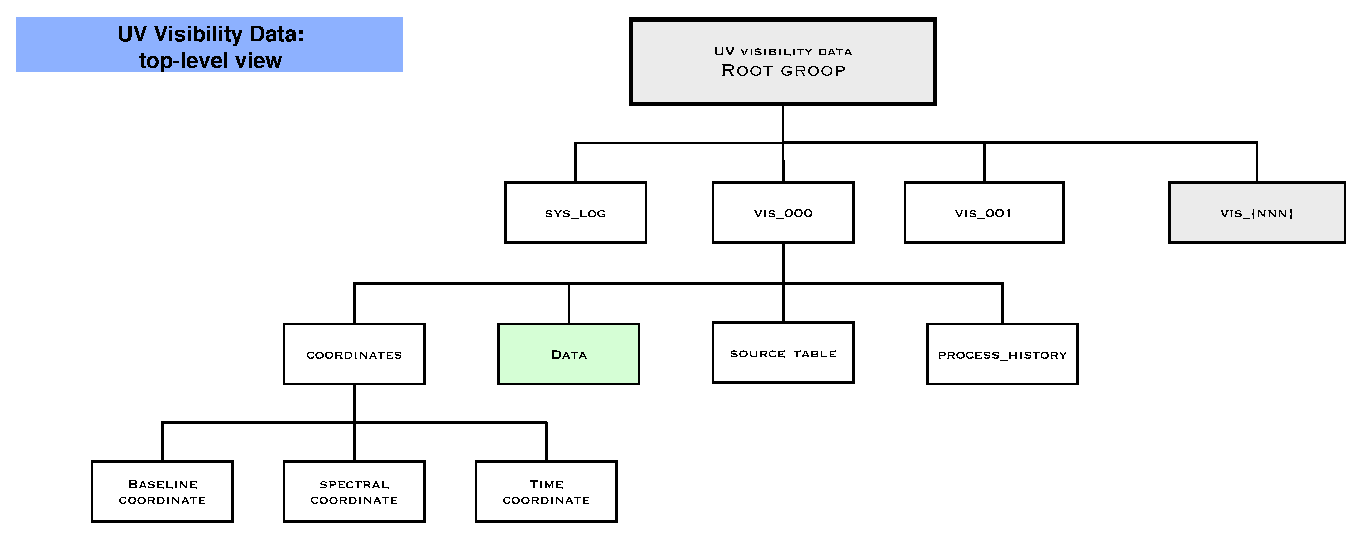
\includegraphics[width=\textwidth]{figures/Vis_TopLevelView.eps}
  \caption{UV Visibility file structure}
  \label{fig:high-level structure}
\end{figure}

This structure can be represented through HDF5 as a \textsc{posix}-style hierarchy:

\begin{verbatim}
OBSERVATION/
OBSERVATION/SysLog
OBSERVATION/Vis001/Coordinates
OBSERVATION/Vis001/Coordinates/<DirectionCoord>
OBSERVATION/Vis001/Coordinates/<LinearCoord>
OBSERVATION/Vis001/Coordinates/<SpectralCoord>
OBSERVATION/Vis001/Coordinates/<TabularCoord> 
OBSERVATION/Vis001/Coordinates/<PolarizationCoord>
OBSERVATION/Vis001/Data
OBSERVATION/Vis001/Source
OBSERVATION/Vis001/ProcessHist
...
OBSERVATION/VisNNN/...
OBSERVATION/MashedVISImages/
...
\end{verbatim}

\subsection{Overview of UV Visibility Groups}

A LOFAR UV Visibility file will then comprise \texttt{System Log
  Group} just below the root level which contains logs and parameter
files which are relevant to the entire file.  Additionally, just below
the root level, the UV Visibility file will contain an arbitrary,
observation-dependent number of \texttt{Vis Groups} containing a
\texttt{Coordinates Group}, a \texttt{Source Group}, and a
\texttt{Processing History Group}, which contains pertinent logs and
parameter sets of the relevent UV Visibilty sub-band.

These main building blocks of the UV Visibility HDF5 file are:

\begin{enumerate} \parskip 0pt
\item \textbf{File Root Group} (\verb|ROOT|). The root level of the file contains
  the majority of associated meta-data, describing the circumstances
  of the observation. These data attributes include time, frequency
  and other important characteristics of the dataset. See
  Sec.~\ref{sec:root group} for a detailed description.
  
\item \textbf{System Logs Group} (\verb|SYS_LOG|). This is a catch-all
  envelop encapsulating information about all the system-wide steps of
  processing which are relevant to the entire observation, such as
  parameter sets and processing logs. See Sec.~\ref{sec:sylog group}
  for a detailed description.

\item \textbf{Vis Groups}. Each observation sub-band is stored as a
  seperate group within the file, containing its own set of four (4)
  sub-groups.  Characteristics about each sub-band uv visibility are
  stored as Attributes in group headers.  LOFAR imaging can produce up
  to 248 sub-bands, which will be the maximum number of uv visibilty
  groups possible in a LOFAR UV Visibility.  Each uv visibility group
  will contain one Data group, which will in turn contain (1) dataset
  as an ndarray, along with associated attributes.

\item \textbf{Source Groups}.  Each observation sub-band processing
  produces a file describing what is called the Local Sky Model (LSM).
  A \textbf{Source Group}  will contain a table of the sources listed
  in a processing file, a \verb|.skymodel| file. Attributes will described
  the columnar data. 

\item \textbf{Coordinates Groups} (\verb|COORDINATES|). Each
  \texttt{Image Group} contains one \texttt{Coordinates Group}, which
  stores the relevant world coordinate conversions.

\item \textbf{Processing History Groups} (\verb|PROCESS_HISTORY|)
  can be found on the \texttt{Image Group} level. These are catch-all
  envelops encapsulating information about all the steps of
  processing, such as parameter sets and processing logs. See
  Sec.~\ref{sec:processing history group} for a detailed description.

\item \textbf{UV Vis Sub-band Data arrays}. For each Vis Group, the
  subband uv visibility data are stored as ndarrays in the respective
  Data group -- it is at this 4th hierarchical depth that the bulk of
  the data reside. The data storage options are still being
  investigated, in order to determine the maximum efficiency of data
  seeks and file I/O.
\end{enumerate}

%% _______________________________________________________________________________
%% Detailed Data Specification

\section{Detailed Data Specification}
\label{sec:detailed structure}

\input metadata_intro

\subsection{The Root Group ({\tt ROOT})}
\label{sec:root group}

The LOFAR file hierarchy begins with the top level \textbf{File Root
  Group} (\verb|ROOT|). This is the file entry point for the data, and
the file node by which navigation of the data is provided.  The
\textbf{File Root Group} will comprise a set of attributes that describe
the underlying file structure, observational metadata, the LOFAR Visibility Data
data, as well as providing hooks to all groups attached to the
\textbf{File Root Group}.

This section will specify two set of attributes that will appear in
the \texttt{Root Group}: a set of Common LOFAR Attributes (CLA) that
will be common to all LOFAR science data products, and a set of
attributes that are specific to LOFAR UV visibility data. Though
these attributes will all appear together in the \texttt{Root}
attribute set, they are separated in this document in order to
demarcate those general LOFAR attributes that are applicable across
all data, and those attributes that are visibility-specific.

In other words,
\begin{verse}
  \verb| Root Attributes = Common LOFAR Attributes + Supplemental UV Vis Root Attributes.|
\end{verse}

The Common LOFAR Attributes are the first attributes of any LOFAR file root group.

\subsubsection{Common LOFAR Attributes}
\label{sec:LOFARCommonMetadata}

Table 2 lists the Common LOFAR Attributes (CLA) which can be found in
LOFAR observation mode data types: Beam-Formed, Transient Buffer Board
(TBB) dumps, Time-series, and imaging, within the files' root
header. These Attributes are required to be in the Root Group; if a
value is not available for an Attribute, a \verb|`NULL'| maybe used in
its place.

\begin{list}{\textbf{--}}{}
\item  \verb|GROUPTYPE| -- The first Attribute in every group must be
  the attribute (\verb|GROUPTYPE|).  Since the CLA are in the root
  header, the value in the CLA for (\verb|GROUPTYPE|) = `Root'.  The
  options for the group type are listed in the Group Type table below,
  grouped by category.
\begin{table}[ht]
  \centering
  \begin{tabular}{|lrp{6cm}|} 
    \hline
    \sc \textbf{General LOFAR Group} & \sc \textbf{Value} & \textbf{Description} \\
    \hline
    Root            & \verb|`Root'|              & Top-level LOFAR group type \\
    System Log & \verb|`SysLog'|          & System log files, parsets \\
    Average Vis & \verb|`MashedUVVis'|& Summed uv visibility\\
   \textbf{Vis}  & \verb|`Vis'|                & Vis group \\
    \hline \hline
    \sc \textbf{Vis Group Subgroups} & \textbf{Value} & \textbf{Description} \\
    \hline
    Data group  & \verb|`Uvvis'| & This is a UV Visibility Data group \\
    Source group & \verb|`Source'| & This is a Source List group \\
    Processing History group &\verb|`ProcessHist'| & This is a Processing History group \\
    Masks group* & \verb|`Masks'| & This is a Masks group \\
    \textbf{Coordinates Group} & \verb|`Coordinates'| & This is a Coordinates group \\
    \hline
    \sc \textbf{Coordinates Group Subgroups} & \textbf{Value} & \textbf{Description} \\
    \hline
    Direction coord group &\verb|`DirectionCoord'|& This is a direction coord group \\
    Linear coord group      &\verb|`LinearCoord'|      & This is a linear coord group \\
    Spectral coord group   &\verb|`SpectralCoord'|  & This is a Spectral coordinate group \\
    Tabular coord group    &\verb|`TabularCoord'|    & This is a tabular coord group \\
    Polarization coord group     &\verb|`PolarizationCoord'|      & This is a Polarization coordinate group \\
    \hline
     *\textit{Proposed groups under advisement.} & & \\\hline \hline
   \end{tabular}
  \label{tab:group type}
  \caption{LOFAR UV Visibility Group Types}
\end{table}
\end{list}

\input lofar_common_metadata

\subsubsection{Supplemental UV Visibility Root Attributes} The root
group of a LOFAR UV Visibility file will comprise header attributes,
various subgroups as indicated above, and appropriate pointers to
root-level an arbitrary number of \verb|Vis| sub-groups, wherein each
Vis group comprises the relevent data and meta-data for a single
sub-band of an observation.

 This root group header will comprise general information about the
 observation itself, sparing relevant data details for the headers of
 the lower order sub-groups.  Table \ref{tab:attributes root group}
 presents additional root group attributes for a LOFAR UV Visibility
 file that do not appear in the LOFAR common metadata
 table.\footnote{\textbf{ *} Indicates attributes that may
   \textit{migrate from the root group} and be broadcast to individual
   \texttt{Vis} groups.  Recent observations have indicated that
   different sub-bands potentially can have different integration
   times.}

\begin{table}[htbp]
  \centering
  \begin{tabular}{|llrl|}
    \hline 
    \sc Field/Keyword     & \sc Type     & \sc Value & \sc Description \\
\hline \hline 
\small{\verb|VISGROUPS|}         & bool  &\verb|`true'| & File has uv visibility subgroups \\
\small{\verb|NOF_IMAGES|}       & int    &  & \small{\texttt{N}} Vis groups in this file \\
\small{\verb|RA_TARG |}         & float  &   & \small{\texttt{RA}} of \small{\texttt{TARGET}} (at LOFAR core)\\
\small{\verb|DEC_TARG|}         & float  &   & \small{\texttt{Dec}} of \small{\texttt{TARGET}} (at LOFAR core)\\
\small{\verb|ORIGFILE|}         & string &    & Input data file (MS?) \\   
\hline
\end{tabular}
\caption{Additional Root group attributes, LOFAR UV Visibility}
\label{tab:attributes root group}
\end{table}

\subsection{The Vis Group}
\label{sec:image group}

The \texttt{Vis} group will be an HDF5 group serving as a container
for the four sub groups described below. As far as is posssible, an
\texttt{Vis} group is designed to be a complete and self-contained
package of uv visibility data.  It will contain relevant data and
metadata for a particular processed sub-band of a LOFAR observations.
However, any breakout protocol will be required to inherit some or all
root group attributes in order to function as a stand-alone image.
The adopted form allows for relatively simple extraction and
conversion in a FITS-compatable form.

\begin{itemize}
\item A \texttt{Coordinates} group that will contain one or more
  subgroups of kinds \texttt{LinearCoord, TabularCoord, SpectralCoord,
    DirectionCoord, PolarizationCoord}, that will describe various
  axes of the associated dataset.
\item A \texttt{Data} group that will contain a dataset array.
\item A \texttt{Source} group that will be a tabular representation of
  a Local Sky Model.
\item A \texttt{ProcessHist} group, which will be a meta-data
  container holding various processing products such as log files,
  parameter sets, RFI mitigation tables, etc.
\end{itemize}

\textit{Figure 2} illustrates the form of an Vis group in a LOFAR UV Visibility file.  The table of Vis group attributes is notably sparse here and the reader must bear in mind that the Coordinates groups will contain most of the rest of the relevent Vis group metadata (\textit{see \ref{sec:coordinates group}, ``Coordinates group''})

\begin{table}[ht]
  \centering
  \begin{tabular}{|llll|}
    \hline
    \sc Field/Keyword & \sc Type & Value &\sc Description \\
    \hline \hline
    \small\verb|GROUPTYPE|       & \verb|string| & \verb|`Vis'| & \small{\texttt{LOFAR}} group type \\
    \small\verb|COORDINATES|     & \verb|string| &   & name of \verb|`Coordinates'| subgroup  \\
    \small\verb|DATAGROUP|       & \verb|string| &   & name of \verb|`Data'| subgroup \\
    \small\verb|SOURCEGROUP|     & \verb|string| &   & name of \verb|`Source'| subgroup \\
    \small\verb|PROCESS_HISTORY| & \verb|string| &   & name of \verb|`ProcessHist'| subgroup \\   
    \hline
  \end{tabular}
  \label{tab:Vis group Attributes}
  \caption{Vis group Attributes}
\end{table}


\subsection{The Coordinates Group}
\label{sec:coordinates group}

Coordinate information within a LOFAR UV Visibility file will exist in what is called a \texttt{Coordinates} group, which will act as a container for a number of \texttt{Coordinates} group objects.  The \texttt{Coordinates} group will be a subgroup of an \texttt{Vis} group container, and may contain one or more subgroups that will describe relevent axes of the coordinates' associated \texttt{Data} group using one or a combination of coordinate subgroups, where the enumerated are \texttt{direction, linear, tabular, spectral, polarization}.

\input coordinates_group_table

The attributes, as presented in Table \ref{tab:coordinates-group},  summarize the
overall characteristics of the set of coordinates collected within this group:
\begin{itemize}
\item \verb|GROUPTYPE| -- Identifier for the type of group, ``Coordinates''.
\item \verb|NOF_COORDINATES| -- The number of coordinate objects/groups contained within the coordinates group.
\item \verb|NOF_AXES| -- The number of coordinate axes associated with the 
  coordinate objects. Keep in mind, that a coordinate can have multiple (coupled)
  axes:  e.g. a direction coordinate is composed of two axes.
\end{itemize}

The layout of the embedded sub-groups will depend on the type of coordinate, of
which there are several types.

\subsubsection{Linear coordinate}
\label{sec:coord-linear}

\input coordinates_coord_linear

\subsubsection{Spectral coordinate}
\label{sec:coord-spectral}

\input coordinates_coord_spectral

\subsubsection{Polarization coordinate}
\label{sec:polarization coordinate}

\input coordinates_coord_polarization

\subsubsection{Tabular coordinate}
\label{sec:coord-tabular}

\input coordinates_coord_tabular

\subsection{The Data Group}

A \texttt{Data} group will most often be a subgroup of an \texttt{Vis} group  container and consist of an HDF5 ``dataset,'' which, as defined in the HDF5 documentation (\textit{see \S\ References}), is ``stored in two parts: a header and a data array.''  However, with the adoption of a so-called ``Coordinates group,'' which contains all the relevent pointing, projection, and unitary information, scale and unit metadata, \texttt{Data} group attributes will be limited. 

LOFAR UV Visibility files will limit attributes to nominal keyword-value pairs as much as possible, with a thought toward potential future user requests for FITS format images.  See \S\ \ref{sec:coordinates group} ``The Coordinates group,'' for a detailed specification of \texttt{Data} group header attributes.

\begin{table}[ht]
  \centering
  \begin{tabular}{|lllrl|}
    \hline
    \sc Field/Keyword & \sc H5Type & \sc Type & \sc Value & \sc Description \\
    \hline \hline
    \small{\verb|GROUPTYPE|}   & Attribute & string &\verb| 'Data'|& Group type descriptor \\
    \small{\verb|DATASET|}       & Attribute & bool   &\verb| 'true'| & the group contains a data array \\
   \small{\verb|WCSINFO|}       & Attribute & string &\verb| '/Coordinates'| & hdf5 path to Vis group WCS data \\
    \hline
  \end{tabular}
\end{table}

The dataset array will (usually) be a ndarray data structure, as can be created by the Python \textit{numarray/numpy} packages. The nominal dimensionality of a \texttt{Data} group's dataset will be 4 (\texttt{NAXIS=4}), wherein the image cube (or cubes) will be defined in (C-type order) \textit{Polarization}, \textit{Frequency}, \textit{Dec}, \textit{RA}, 

\begin{center}
  \begin{tabular}{|llll|}
    \hline
    \textsc{Vis} & \textsc{Quantity} & \textsc{Axes} & \textsc{Units} \\
    \hline \hline
    Sky image & $I (p, \nu,\mathrm{Dec},\mathrm{RA})$      & Pol/Freq/Dir/Dir                       & .. /Hz/deg/deg  \\
       RM cube & $RM (p, \phi,\mathrm{Dec},\mathrm{RA})$ & Pol/Faraday Rot/Dir./Dir.          & .. /rad m$^{-2}$/deg/deg \\
       RM map  & $RM (\mathrm{Dec},\mathrm{RA})$            & Dir./Dir.                                     &    /deg/deg \\
     CR image  & $I(p, \nu,r,\mathrm{El}\mathrm{Az})$        & Pol/Freq/Dist/Dir./Dir./            & .. /p/Hz/m/deg/deg \\
     CR image  & $I(p, t, \nu, \xi_3, \xi_2, \xi_1)$                 & Pol/Time/Freq/Pos/Pos/Pos     & .. /s/Hz/m/m/m \\
    \hline
  \end{tabular}
\end{center}

\subsection{The Source Group}

The \texttt{Source} group in a UV Visibility file will be a table of sources and their associated parameters.  The \texttt{Source} group header will specify the fields (columns) of the table, the number of sources in the table (rows). See Table \ref{tab:attributes source group} for the specification of \texttt{Source} group attributes for a LOFAR UV Visibility file.

\begin{table}[ht]
  \centering
  \begin{tabular}{|llrl|}
    \hline
    \sc Field/Keyword & \sc Type      & \sc Value & \sc Description\\
    \hline \hline                    
    \small{\verb| GROUPTYPE|} & string &\verb|`Source'| & UV Visibility group type \\
    \small{\verb| DATASET|}   & string &\verb|`Source List'|   & These data are a local sky model \\
    \small{\verb| NAXIS|}     & int       &\verb|2|                   & Number of data axes \\
    \small{\verb| NAXIS1|}    & string &\verb|`Fields'|           & Axis of the data fields \\
    \small{\verb| NAXIS2|}    & string &\verb|`Source'|          & Axis of the source rows. \\
    \small{\verb| NSOURCE|}   & int       &               & Number of data rows/sources \\
    \small{\verb| FIELD1|}    & float   &     & RA (at LOFAR core)\\
    \small{\verb| FIELD2|}    & float   &     & Dec (at LOFAR core)\\
    \small{\verb| FIELD3|}    & float   &     & Peak Flux \\
    \small{\verb| FIELD4|}    & float   &     & Integrated Flux \\
    \small{\verb| FIELD5|}    & float   &     & Gaussian semi-major axis \\
    \small{\verb| FIELD6|}    & float   &     & Gaussian semi-minor axis \\
    \small{\verb| FIELD7|}    & float   &     & Position angle \\
    \hline
  \end{tabular}
  \caption{Attributes of a Source group.}
  \label{tab:attributes source group}
\end{table}

%% _______________________________________________________________________________
%% Subsection: The Processing History Group (PROCESS_HISTORY)

\subsection{The Processing History Group ({\tt PROCESS\_HISTORY})}
\label{sec:processing history group}

The data definition for the \textbf{Processing History Group}
is necessarily loose, and will accommodate a variety of ancillary
meta-data related to or produced by the various LOFAR processing
pipelines. Products such as DPPP log files, processing parameter
sets, RFI mitigation tables, etc., may appear in this group.  In fact,
and due to the wide-ranging data types and free-form ASCII format the
many log files may present, the \textbf{Processing History Group} will
be a catch-all envelop encapsulating information about all steps of
processing should the user need such information.

\input table_processing_history

\begin{figure}[htbp]
  \begin{center}
    \includegraphics{figures/ProcessingGroup2.eps}
 \caption{The processing history group, nested tabulation}
 \end{center}
  \label{fig:processing history group}
\end{figure}

As with all other UV Visibility file HDF5 groups and subgroups, the \texttt{Processing History} group will be an HDF5 group, as a subgroup of an \texttt{Vis} group.
The attributes will contain a brief summary of the appended processing files
contained therein, with pointers to tables containing the logging data, parameter
sets, etc..

%% ------------------------------------------------------------------------------

\section{Interfaces}
\label{sec:interfaces}

---/---

\subsection{Interface requirements}

---/---

\subsection{Relation to other workpackages}

---/---

%% ==============================================================================
%%
%%  Appendices
%%
%% ==============================================================================

\clearpage
\appendix

%%_______________________________________________________________________________
%% Discussion & open questions

\section{Discussion \& open questions}
\label{sec:discussion}

\subsection{Open questions/Issues}
\label{sec:open-questions}

\begin{enumerate}
\item Do we really need a full description of all coordinate types within this
  document? Since this information written down in detail in
  \texttt{LOFAR-USG-ICD-002}, we rather might want to restrict ourselves here
  to the specific metadata used for Visibility data.
\end{enumerate}

\subsection{Future enhancements}
\label{sec:future-enhancements}

---/---

%%_______________________________________________________________________________
%% LOFAR Filename Convention

\section{LOFAR Filename Convention}
\label{sec:filenames}

The LOFAR file naming convention is described in the document,
\texttt{LOFAR-USG-ICD-005} \cite{lofar.icd.005}. Readers are
encouraged to consult that document for specifics on LOFAR file naming
conventions.

%%_______________________________________________________________________________
%% Coordinates group examples

\section{Coordinates group examples}
\label{sec:coordinate examples}

An in-depth description -- including a number of examples -- can be found in
\texttt{LOFAR-USG-ICD-002} \cite{lofar.icd.002}. Readers are encouraged to
consult that document for specifics on the storage of world coordinates
information.

%%_______________________________________________________________________________
%% LOFAR common glossary

\section*{\glossaryname}
\label{sec:glossary}
\addcontentsline{toc}{section}{\glossaryname}

\input lofar_common_glossary

%%_______________________________________________________________________________
%% Bibliography

\bibliographystyle{plain}
\bibliography{references}

\end{document}
